%%%%%%%%%%%%%%%%%%%%%%%%%%%%%%%%%%%%%%%%%%%%%%%%%%%%%%%%%%%%%%%%%%%%%%%%%%%%%
\section{Examples of OpencCL Applications}


%------------------------------------------------------------------------------
\subsection{OpenCL on FPGA platforms}

\subsubsection{OpenCL-FPGA Implementation}
As we already saw, OpenCL applications consists of two part: the host and the kernels.
FPGA flexibility allow the developer to opt for two solutions:

\begin{enumerate}
	\item An "`All in One"' solution, by implementing the CPU that will run the standard C/C++ host code directly as a soft CPU inside the FPGA.
	\item A separate solution, by using an external microprocessor for the host and by programming the FPGA to execute the kernels only.
	\end{enumerate}
	
Unlike CPUs and GPUs, where parallel threads can be executed on different cores, FPGAs offer a different strategy. Kernel functions can be transformed into dedicated and deeply pipelined \textbf{hardware circuits} that are inherently multithreaded using the concept of pipeline parallelism. Each of these pipelines can be replicated many times to provide even more parallelism than is possible with a single pipeline. This translates in an immediate boost in performance.\\
Figure \ref {fig:fpga_example} shows a simple example of how kernels are translated into separate \textbf{hardware pipelines}.
	
\begin{figurehere}
 \centering
 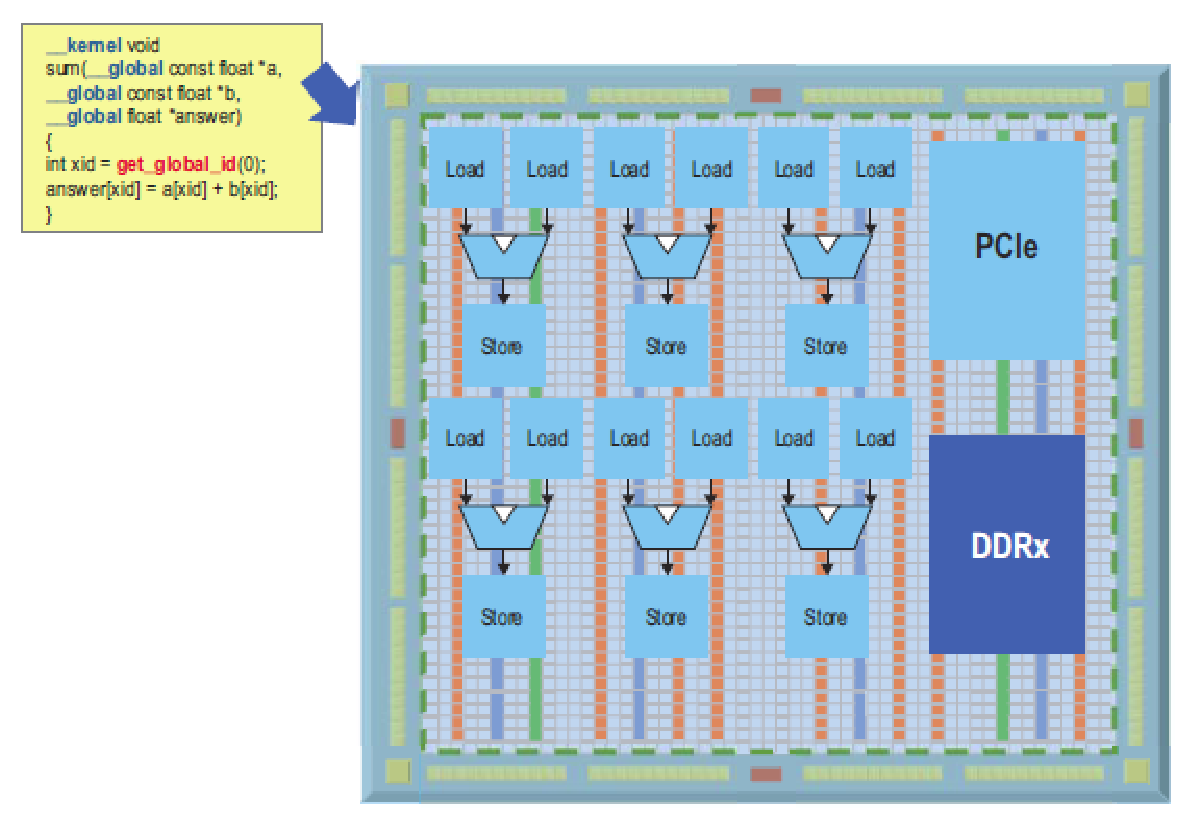
\includegraphics[width=8cm, height=4cm]{./eps/FPGA1.eps}
 \caption{FPGA implementation example}
 \label{fig:fpga_example}
\end{figurehere}

The most important concept behind the OpenCL-to-FPGA compiler is the notion of \textbf{pipeline parallelism}.
Basically, an OpenCL-to-FPGA compiler is able to implement the scenario observed in Section \ref{sect:pipelineScenario} in an automatic and more efficient way. We will describe how pipeline parallelism work by introducing an example, shown in Figure \ref{fig:fpga_example2}:

\begin{figurehere}
 \centering
 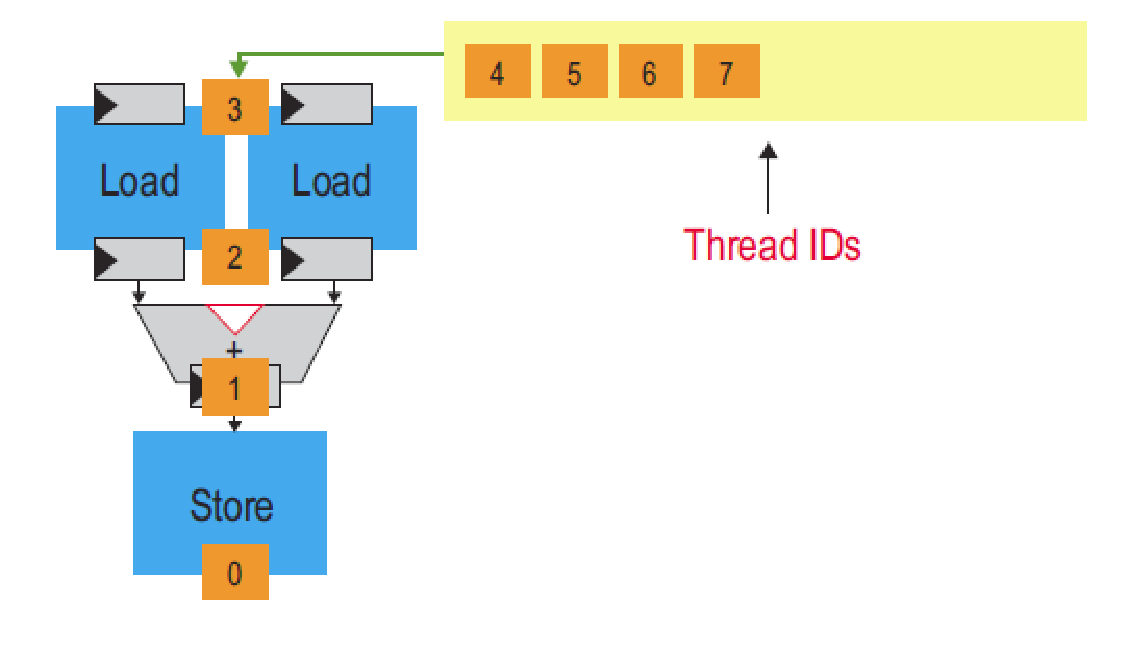
\includegraphics[width=8cm, height=4cm]{./eps/FPGA2.eps}
 \caption{Pipeline parallelism example}
 \label{fig:fpga_example2}
\end{figurehere}

On the first clock cycle, thread 0 is clocked into the two load units. This indicates that they should begin fetching the first elements of data from arrays A and B. On the second clock cycle, thread 1 is clocked in
at the same time that thread 0 has completed its read from memory and stored the results in the registers following the load units. On cycle 3, thread 2 is clocked in, thread 1 captures its returned data, and thread 0 stores the sum of the two values that it loaded. It is evident that in the steady state, all parts of the pipeline are active, with each stage processing a different thread.
	
To complete this section, we'll present a general scheme that summarize how OpenCL-FPGA applications are implemented (Figure \ref{fig:fpga_implementation}). One crucial point for parallel computation is the memory management, and as we can see from the figure several memory interfaces are needed, but luckily OpenCL-FPGA compilers are usually able to implement such interfaces automatically.

\begin{figurehere}
 \centering
 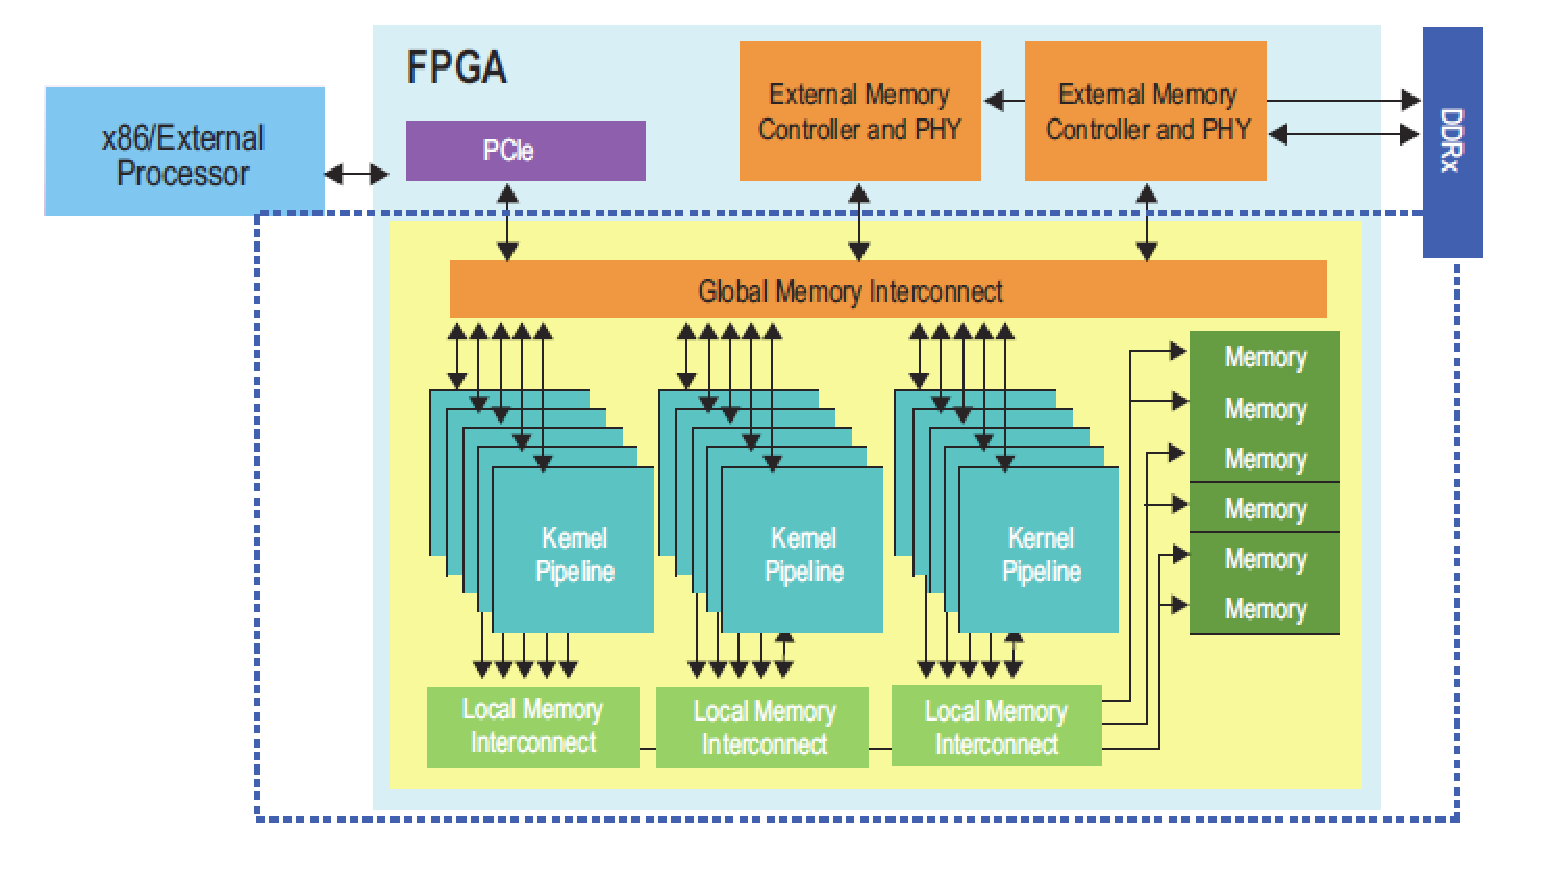
\includegraphics[width=8cm, height=4cm]{./eps/FPGA3.eps}
 \caption{OpenCL-FPGA Implementation scheme}
 \label{fig:fpga_implementation}
\end{figurehere}

\subsubsection{Benefits}

\begin{itemize}
	\item \textbf{Improved Time To Market:} OpenCL offers a quicker and simpler way to implement parallel alghorithms  compared to traditional FPGA development using lower level hardware description language (HDLs) such as Verilog or VHDL \cite {altera:FPGA}.  This because OpenCL inherently offers the ability to describe parallel computation, while the main challenge in HDLs languages was exactly to extract thread-level parallelism from a sequential program. OpenCL offers instead the ability to the programmer to explicitly specify and control parallelism.
	\item \textbf{Better Performance:} Dedicated ad-hoc hardware structures allow faster computation than using generic CPUs. Furthermore OpenCL-FPGA compilers exploit pipeline parallelism to make computation even faster.
	\item \textbf{Less Power Consumption:} Benchmarks show that FPGA applications consumes lot less power to execute the same OpenCL code in comparison to CPU or GPU.
\end{itemize}

\subsubsection{Case Study: Monte Carlo Black-Scholes Method}

In this experiment an economic model was used to benchmark an OpenCL-FPGA unit. The model is based on the 
Monte Carlo Black-Scholes method and it is used to compute the expected payoff of stock prices over millions of different paths. The entire algorithm used for this benchmark can be implemented in approximately 300 lines of
OpenCL code that is portable from FPGA to CPU to GPU, and we can see the comparison in performance on these 3 different platforms in Table \ref{tab:FPGABenchmark}.

\begin{tablehere}
{\footnotesize
\begin{tabular}{|p{1,0cm}|p{1,8cm}|p{1,8cm}|p{1,8cm}|}\hline
\textbf{Platform} & \textbf{Power} [Watts] & \textbf{Performance} [Billions of simulations per seconds] & \textbf{Efficiency} [Millions of sims per second per watt]\\ \hline
CPU & 130 & 0.032 & 0.0025 \\ \hline
GPU & 212 & 10.1 & 48 \\ \hline
FPGA & 45 & 12.0 & 266 \\ \hline
\end{tabular}}
  \caption{Monte Carlo Black-Scholes benchmark results\\}
	\label{tab:FPGABenchmark}
\end{tablehere}

As we can see, not only the OpenCL framework targeting a FPGA board exceeds the throughput of both a CPU and a GPU, but it also consumes one-fifth the power of comparable GPUs when executing the same code.

\subsubsection{Case Study: Document Filtering}

In this benchmark the focus is set on a more practical problem than the previous, as it will consider an algorithm used in modern data centers.
A recent report \cite{walsh:power} from International Data Corporation (IDC) examined the requirements of high performance computing data centers, and conducted a survey of the top constraints in expanding current data center capabilities. From the results, it was obvious that power and cooling costs are the key impediments of compute capability expansion, and as we have seen in the previous benchmark, FPGA computation offer an huge improvement in power consumption over CPUs and GPUs.\\
In this experiment, a document filtering algorithm was implemented using OpenCL, and it basically involves looking at an incoming stream of documents and finding the ones that best match a user's interest. The results are shown in Table \ref{tab:FPGABenchmark2}:

\begin{tablehere}
{\footnotesize
\begin{tabular}{|p{1,0cm}|p{1,8cm}|p{1,8cm}|p{1,8cm}|}\hline
\textbf{Platform} & \textbf{Power} [Watts] & \textbf{Performance} [Million of Terms per seconds] & \textbf{Efficiency} [Millions of Terms per Joule]\\ \hline
CPU & 130** & 2070 & 15.9 \\ \hline
GPU & 215 & 3240 & 15.1 \\ \hline
FPGA & 21 & 1755 & 83.6 \\ \hline
\end{tabular}}
  \caption{Document Filtering benchmark results\\ **Does not include memory consumption.}
	\label{tab:FPGABenchmark2}
\end{tablehere}

As we can see, although CPUs and GPUs can perform better in terms on throughput, the power efficiency of these two platform can be five time lower than the efficiency of FPGAs. It is interesting to note that in this case the performance of the FPGA was limited by the external memory bandwidth, and not by the FPGA itself. With a proper setup, the authors extimate a performance value of 2925 MT/s with the same power consumption, that would raise the power efficiency from 83.6 MT/J to 139,3 MT/J.
These results demonstrate that introducing an FPGA OpenCL implementation of algorithms, could bring a dramatic decrease of power consumption and thus cooling costs in modern data centers.


%-----------------------------------------------------------------------------

\subsection{TROVARE TITOLO}

In the next example \cite{Pennycook2012} we'll analyze how OpenCL was used to re-implement an existing benchmarking algorithm to (NO! IN REALTA' E' PIU' LENTO! Scopo: unico source??)damatically increase its performances. This example is interesting because it also analyzes how the introduction of Device Fission allow to obtain even more considerable speedups.

\subsubsection{Background: the LU algorithm}

LU is an application level benchmark part of the NPB Suite (NAS Parallel Benchmark) that consists in a series of parallel aerodynamic simulations designed by NASA. LU is short for Lower-Upper Gauss-Seidel solver and the algorithm is basically a simplified Navier-Stokes equation solver that uses three-dimensional data grid for its calculations. The size of these data cubes is always N^3, and for the purpose of this example we'll focus only on three specific classes of problems: Class A problems (size 64^3), Class B problems (size 102^3) and Class C problems (size 162^3).
To perform the calculations, each cube of size (n X n X n) is divided into 2D "`slices"' of size (n X n X 1), and each "`slice"' is assigned to a different processor for computation. This algorithm is further optimized used a technique called \textit{k-blocking}; Figure \ref{dataCubes} shows a visual representation of how data is explored, as you can see each block must wait for the adjacent block to be completely computed (black blocks)before they can start.

\begin{figurehere}
 \centering
 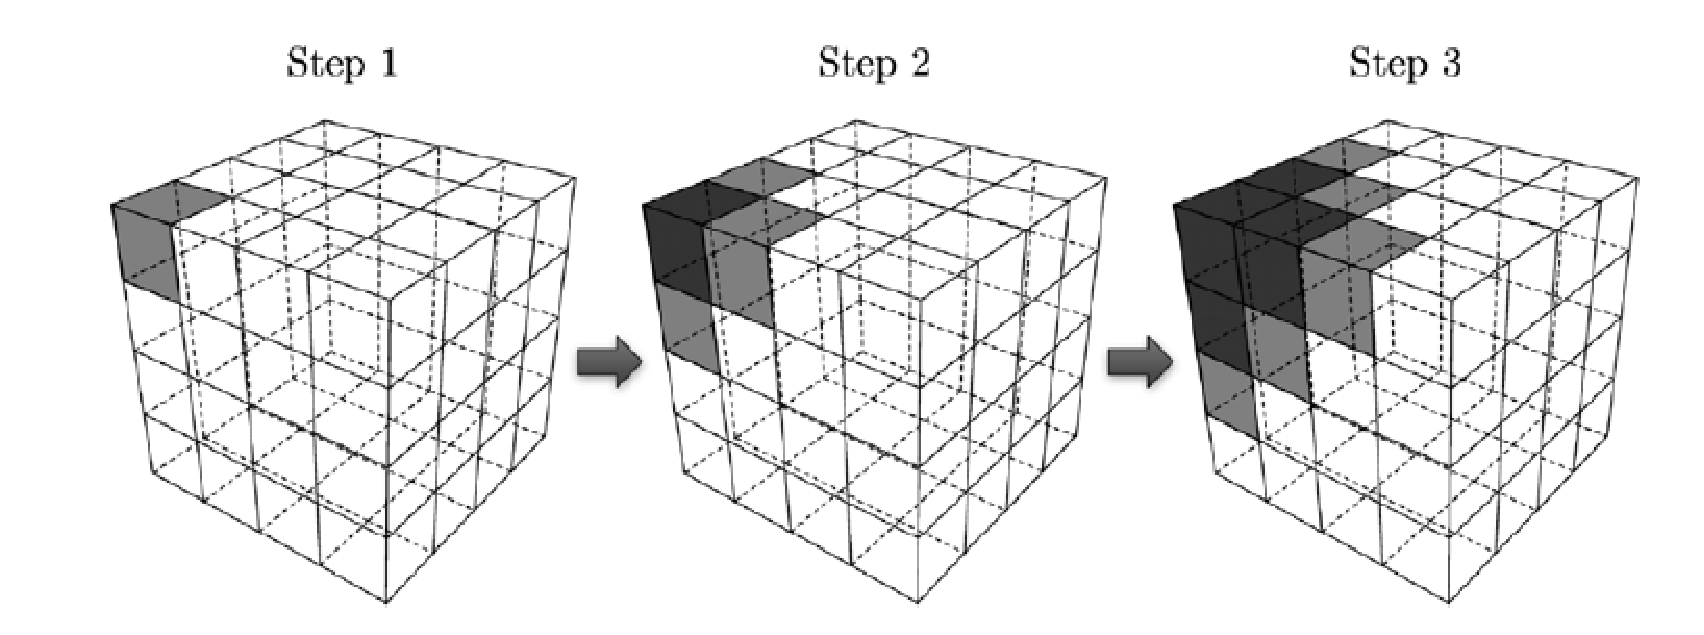
\includegraphics[width=8cm, height=4cm]{./eps/dataCube.eps}
 \caption{Data cubes used in the LU algorithm}
 \label{fig:dataCubes}
\end{figurehere}


\subsubsection{The Experiment}

\begin{tablehere}
{\footnotesize
\begin{tabular}{|p{1,0cm}|p{1,8cm}|p{1,8cm}|}\hline
\textbf{Platform} & \textbf{Compute Units} & \textbf{Processing Elements} \\ \hline
Intel X5550, 2.66 GHz (x86 CPU) & 4 & 4 \\ \hline
Intel X5660, 2.80 GHz (x86 CPU) & 12 & 12 \\ \hline
NVIDIA Tesla C1060 (GPU) & 30 & 240 \\ \hline
NVIDIA Tesla C2050 (GPU) & 14 & 448 \\ \hline
AMD/ATI FirePro V7800 (GPU) & 18 & 1440 \\ \hline
\end{tabular}}
  \caption{Platform used for the experiment}
	\label{tab:LUBenchmark1}
\end{tablehere}

Table \ref{tab:LUBenchmark1} shows a list of devices used in the experiment. One important aspect to note of OpenCl is its code portability: a single source can be used on different devices with different numbers of cores processing units, as OpenCL is able to scale automatically. This, for starters, already offers many benefits:

\begin{itemize}
	\item it is easier to maintain a single code that targets all platforms, as opposed to separate hand-tuned versions of the same code for each alternative platform.
	\item it reduces the risk of being locked into a single vendor solution.
	\item benchmarking is simplified, as the results can be compared from a single code source.
	\item it represents a "`safer"' investment for computing sites, as new codes (and ported legacy codes) will run on both existing and future architectures.
\end{itemize}

The goal of the experiment was to consider the performances of OpenCL implementation of LU against native FORTRAN77 (for CPUs) and CUDA (for GPUs). Figure \ref{fig:OpenCLvsFORTRAN77} shows the results for the comparison of the OpenCL implementation against the native FORTRAN77 implementation compiled using different compilers.

\begin{figurehere}
 \centering
 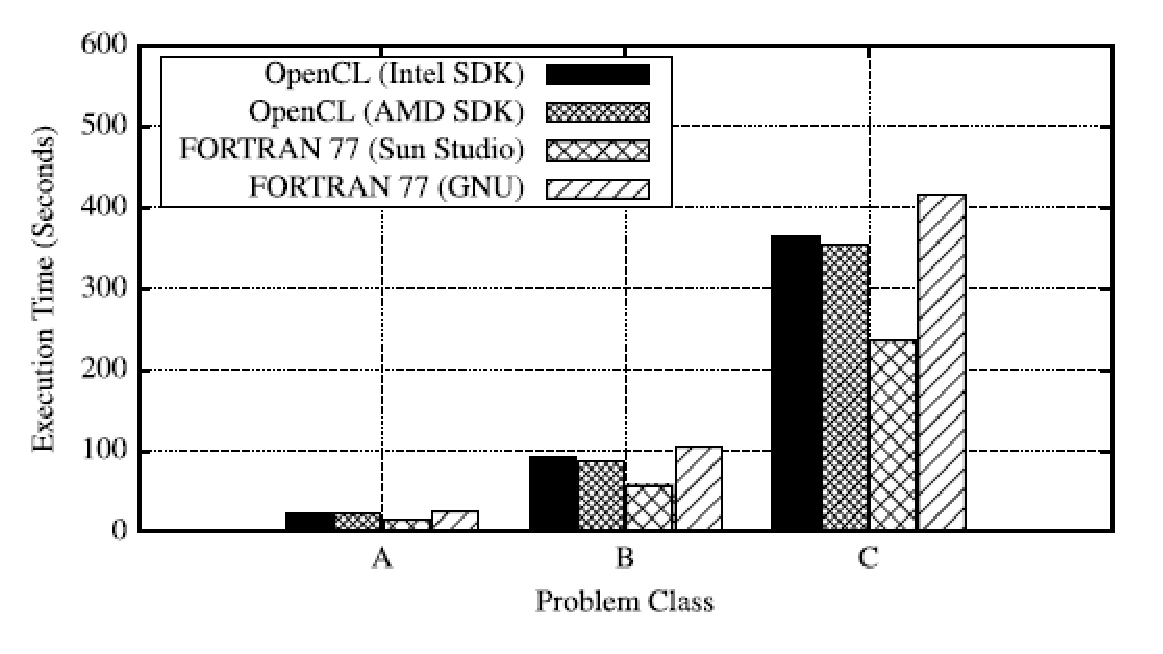
\includegraphics[width=8cm, height=4cm]{./eps/OpenCLvsFORTRAN77.eps}
 \caption{OpenCL vs Fortran Comparison}
 \label{fig:OpenCLvsFORTRAN77}
\end{figurehere}

As we can see the advantage of OpenCL (if any) is very marginal, and in the case of the Sun Studio compiler, the FORTRAN77 implementation performs way better. This result is very interesting because it demonstrates that \emph{OpenCL is not always the best option in term of performance}. The reason of this ``failure'' could be attributed to the fact that the FORTRAN compiler is very mature and has a long story of optimizations and fine-tuning behind it, while OpenCL standard is quite young.
Let's now see how OpenCL perform against another GPGPU implementation (CUDA), the results are shown in Figure \ref{fig:OpenCLvsCUDA}:

\begin{figurehere}
 \centering
 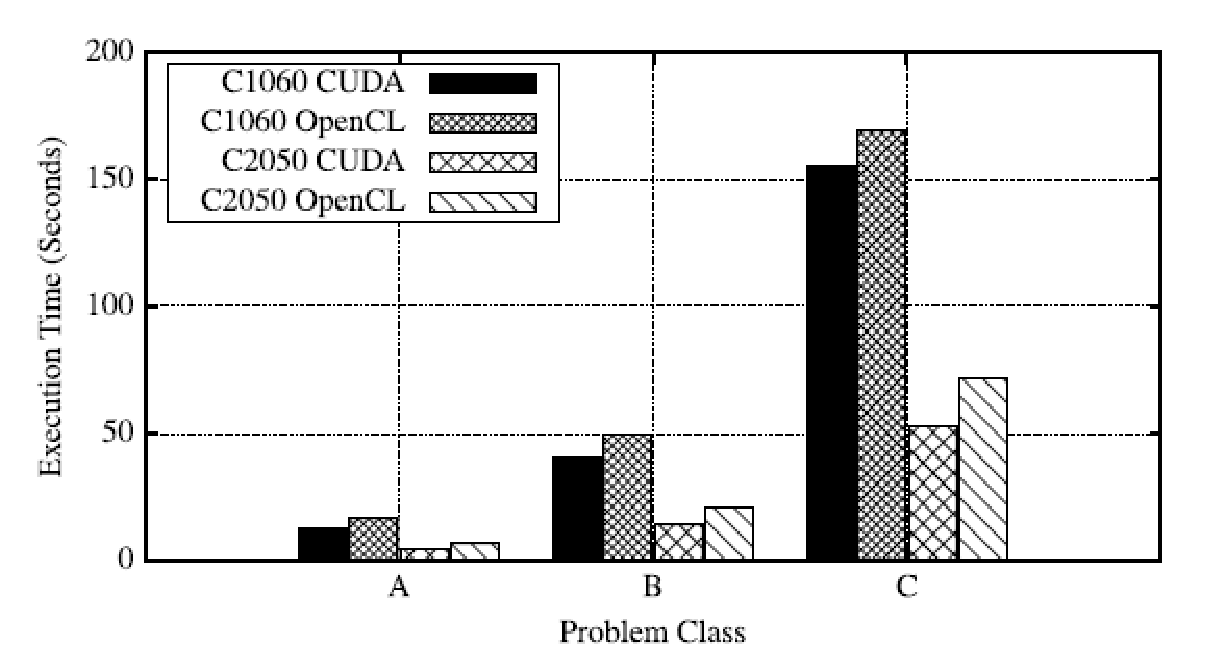
\includegraphics[width=8cm, height=4cm]{./eps/OpenCLvsCUDA.eps}
 \caption{OpenCL vs CUDA Comparison}
 \label{fig:OpenCLvsCUDA}
\end{figurehere}

As we can see even in this case the CUDA implementation performs a little better, and the reason in still to be searched into specific optimizations offered by the CUDA compiler for NVIDIA boards.

\subsubsection{Introducing Device Fission}








